\chapter{Fundamentos Teóricos y Contextuales de la Transformación de Datos Históricos y Sistemas Multiagentes Conversacionales}
\label{chap:chapter1}

\section*{Introducción}
\addcontentsline{toc}{section}{Introducción}

El primer capítulo de la tesis establece el marco teórico, contextual y técnico necesario para el desarrollo de un sistema multiagente conversacional capaz de interactuar con datos históricos del transporte marítimo, extraídos del Diario de la Marina, un periódico cubano de gran relevancia histórica, publicado entre 1844 y 1960. Este capítulo se organiza en torno a cinco pilares fundamentales: la fundamentación teórica del tema, un análisis del estado del arte y del mercado en el ámbito de los sistemas multiagente aplicados a este tipo de contextos, la justificación metodológica del proceso de desarrollo de software, la selección y descripción de las herramientas y tecnologías utilizadas, y la gestión de bases de datos requerida para el procesamiento de la información histórica. Como cierre, se presentan observaciones preliminares que no solo resumen los hallazgos iniciales, sino que también sientan las bases conceptuales y técnicas para los capítulos subsiguientes de la investigación.

\section{Fundamentación Teórica}\label{seq_0}

\subsection{Reconocimiento Óptico de Caracteres (OCR)}\label{seq_1}

El Reconocimiento Óptico de Caracteres (OCR) es una tecnología que permite convertir documentos físicos, como imágenes escaneadas o fotografías de texto, en datos digitales editables. Este proceso emplea algoritmos avanzados para analizar la estructura visual de una imagen, identificando caracteres y palabras a partir de patrones reconocibles, lo que transforma contenido analógico en un formato susceptible de edición, búsqueda y análisis automatizado~\cite{piryani2025multilocraqa}. En el ámbito de la digitalización masiva de archivos históricos, como el \textit{Diario de la Marina} (1844–1960), el OCR desempeña un papel crucial como el primer paso para preservar y dar acceso a un patrimonio cultural que, de otro modo, permanecería confinado a soportes físicos deteriorados.
Sin embargo, su aplicación a documentos históricos no está exenta de limitaciones. Factores como la diversidad de tipografías antiguas, el desgaste físico de los originales y la calidad variable de impresión introducen errores significativos en la transcripción, resultando en datos digitales no estructurados que carecen de organización y metadatos estandarizados. En el caso del \textit{Diario de la Marina} (ver Figura \ref{fig:Diario de la Marina 1884}), estas imperfecciones se evidencian en la conversión de información sobre transporte marítimo —rutas, puertos, cargamentos y fechas—, cuya heterogeneidad dificulta su análisis sistemático.

\begin{figure}[h]
	\centering
	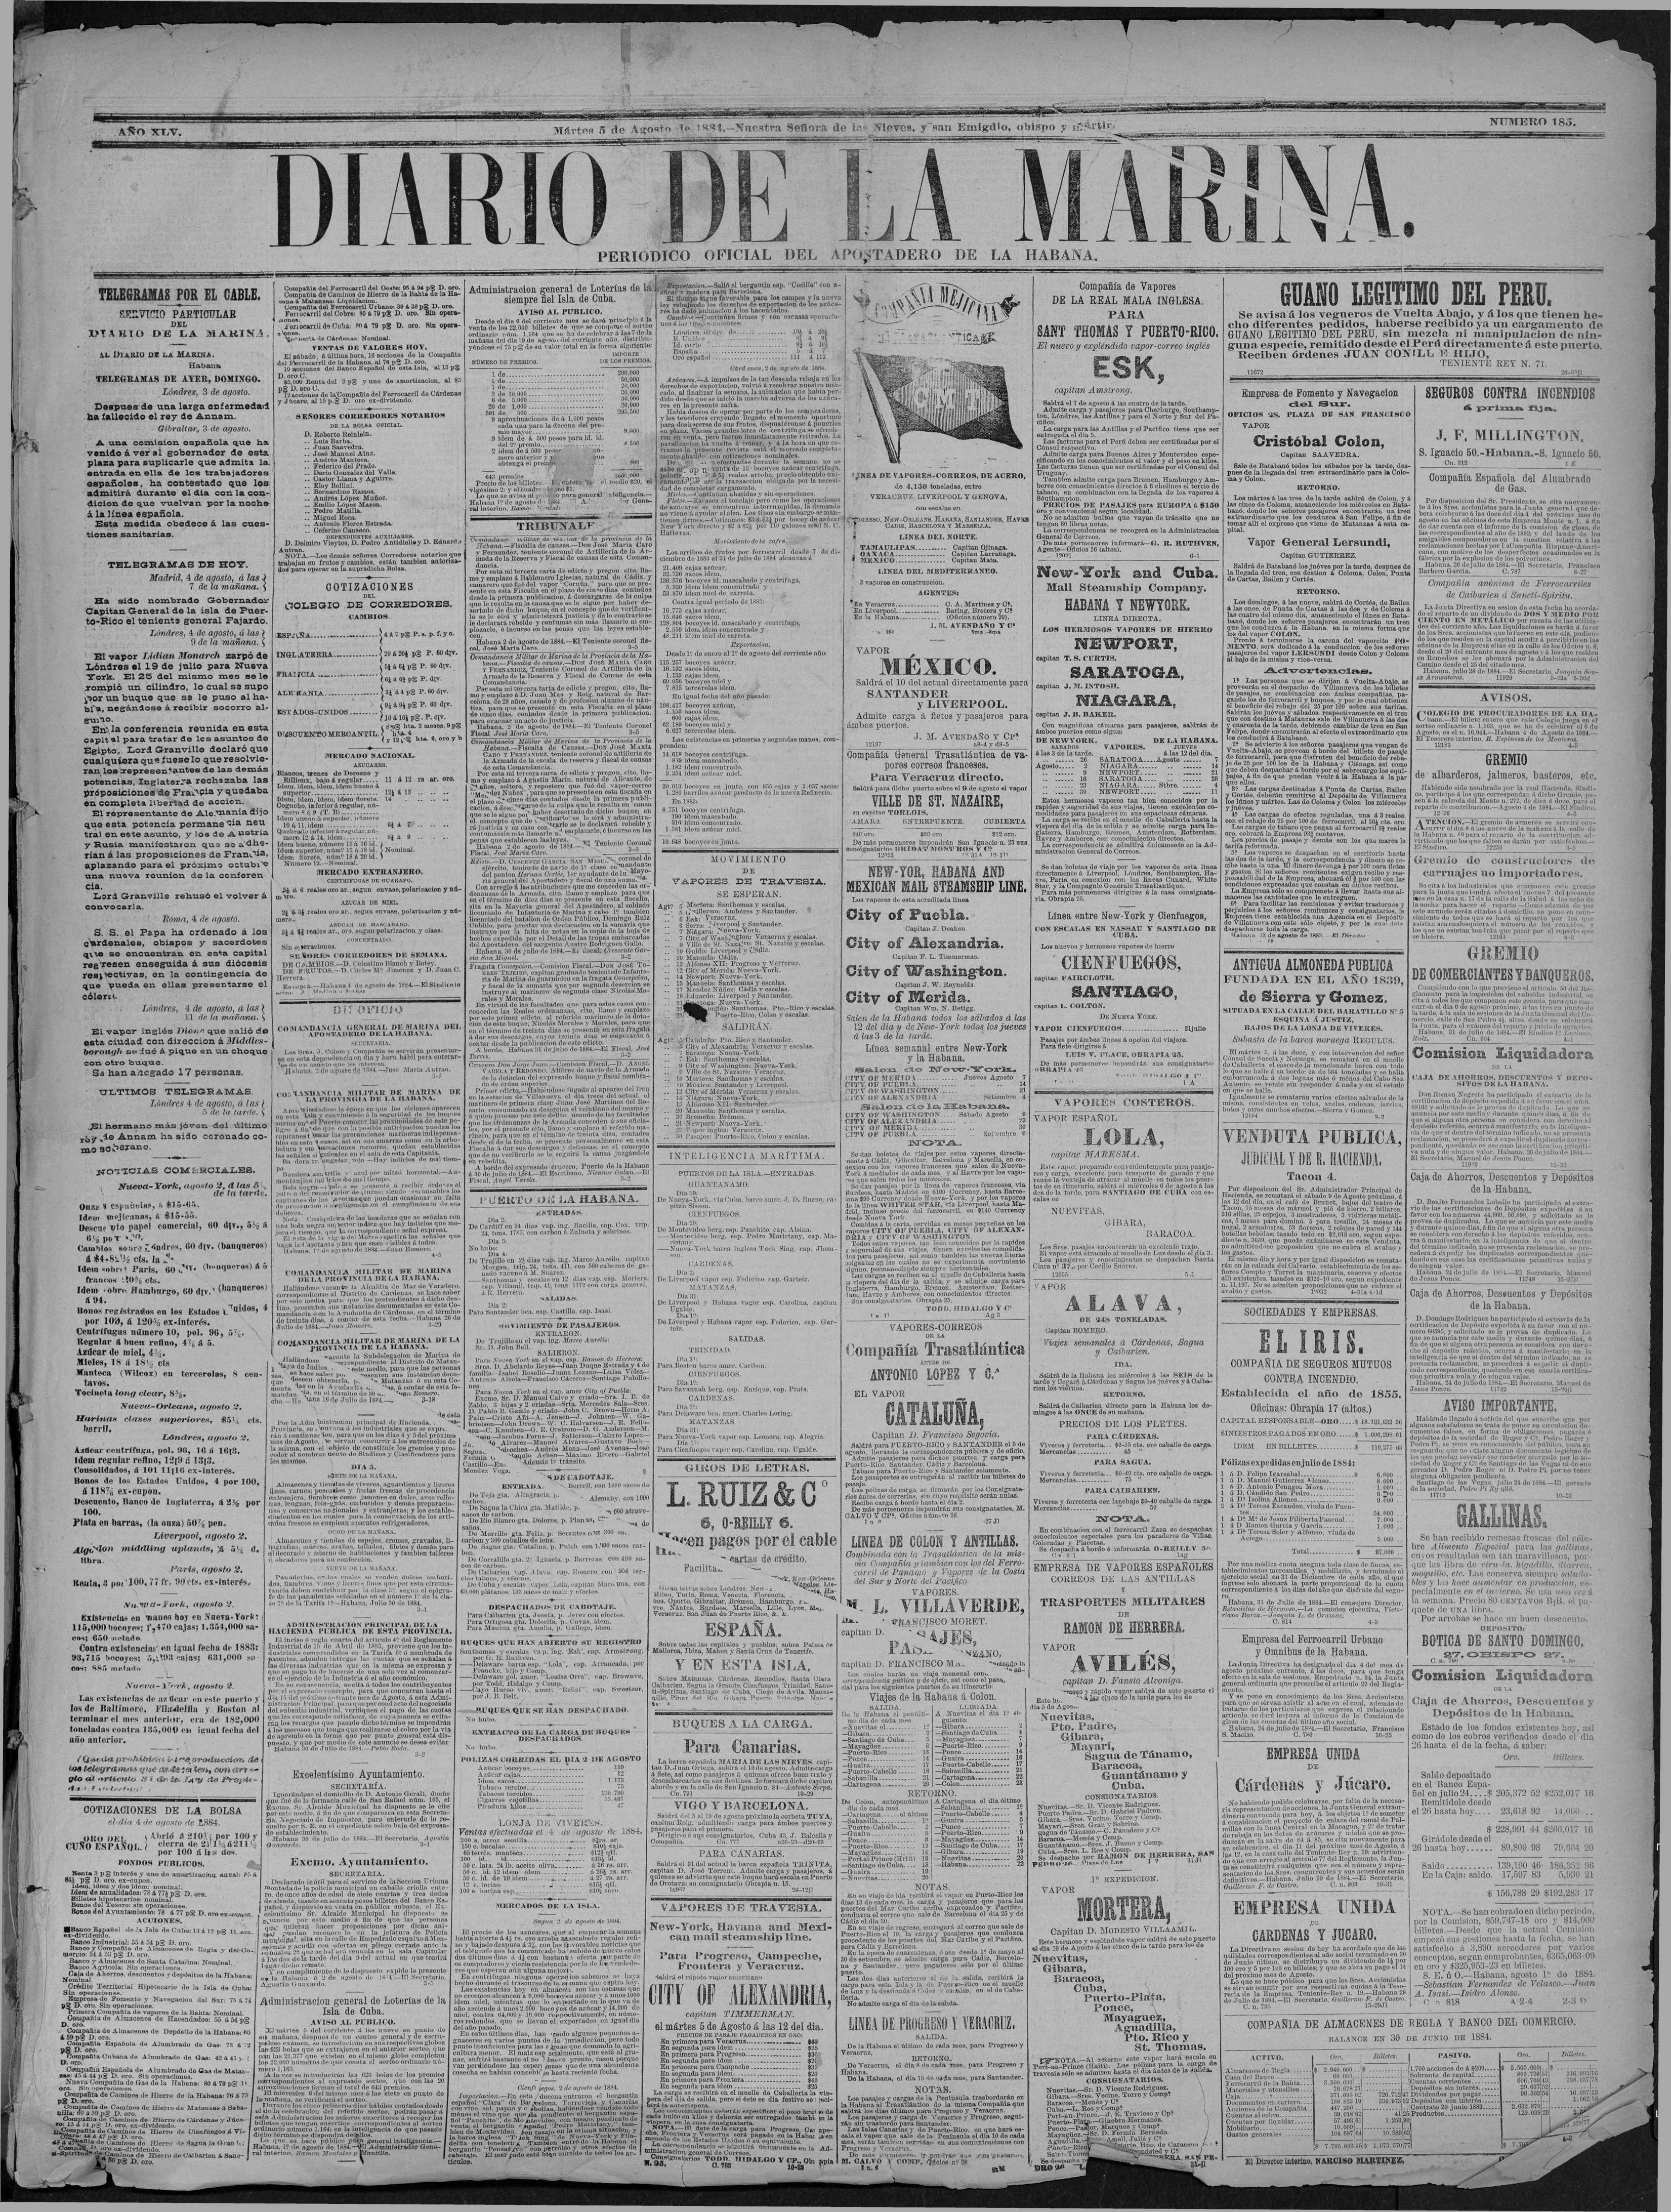
\includegraphics[width=0.3\textwidth]{images/diario}
	\caption{Diario de la Marina 1884.}
	\label{fig:Diario de la Marina 1884}
\end{figure}

La importancia del OCR en esta investigación se deriva de su rol como el primer eslabón en la transformación de estos documentos en datos digitales accesibles, aunque sus limitaciones resaltan la necesidad de enfoques posteriores de inteligencia artificial para refinar y dar sentido a la información resultante.

\subsection{Agente LLM}\label{seq_3}

Los datos generados por el OCR, aunque accesibles, presentan desafíos que requieren herramientas más avanzadas para su interpretación. Aquí es donde entran en juego los agentes basados en modelos de lenguaje de gran escala (LLM, por sus siglas en inglés: Large Language Model), entidades computacionales que aprovechan técnicas de inteligencia artificial para comprender, generar e interactuar con el lenguaje humano de forma sofisticada~\cite{guo2024largelanguage}. Entrenados con vastos conjuntos de datos textuales, estos agentes son capaces de procesar lenguaje natural con coherencia y contextualidad, interpretando significados implícitos y adaptándose a diferentes estilos de comunicación.
En el contexto del Diario de la Marina, los agentes LLM pueden abordar la ambigüedad y los errores de los datos no estructurados producidos por el OCR. Por ejemplo, podrían corregir términos náuticos mal transcritos o inferir el significado de frases incompletas causadas por el deterioro del papel, como una referencia a un cargamento de azúcar en un puerto específico. Además, su capacidad para integrar información externa —mediante herramientas como bases de datos históricas— permite conectar datos aislados con contextos más amplios, como eventos comerciales del Caribe~\cite{guo2024largelanguage}. Este concepto es fundamental porque transforma texto crudo en contenido más comprensible, aunque su acción aislada no basta para estructurar sistemáticamente grandes volúmenes de información histórica, lo que lleva a explorar enfoques más coordinados.


\subsection{Sistema Multiagente (SMA)}\label{seq_2}

Mientras los agentes LLM ofrecen una poderosa herramienta para interpretar texto, la complejidad y el volumen de los datos del Diario de la Marina demandan un enfoque más estructurado. Un sistema multiagente (SMA) se define como un conjunto de agentes autónomos que operan en un entorno compartido, interactuando entre sí para resolver problemas complejos o cumplir tareas específicas que exceden las capacidades de un solo componente~\cite{zambrano2020multiagent}. Estos agentes trabajan de manera independiente pero también colaboran o compiten según los objetivos establecidos, lo que los hace idóneos para manejar información diversa y dinámica~\cite{perezpons2021brief}.
La relevancia de los SMA radica en su capacidad para descomponer la heterogeneidad de los datos históricos en tareas manejables. Por ejemplo, un agente podría especializarse en identificar nombres de puertos en textos mal transcritos, mientras otro contextualiza esos datos con rutas comerciales del siglo XIX. Esta modularidad permite procesar eficientemente grandes volúmenes de información y adaptarse a las particularidades de los documentos históricos. Características como la autonomía, la interacción mediante protocolos como el lenguaje ACL, y la adaptabilidad~\cite{perezpons2021brief}, junto con elementos como agentes, entorno, comunicación y organización~\cite{zambrano2020multiagent}, potencian las capacidades individuales de herramientas como los LLMs, abriendo la puerta a procesos más robustos de análisis y estructuración de datos.

\subsection{Sistemas RAG}\label{seq_4}

La coordinación de agentes en un SMA amplifica su potencial, pero la precisión y relevancia de la información procesada dependen de acceder a contextos actualizados y verificables. Los sistemas RAG (Retrieval Augmented Generation) representan una arquitectura innovadora que combina modelos de lenguaje avanzados con mecanismos de recuperación de información en tiempo real~\cite{gao2024retrievalaugmented,lewis2020retrievalaugmented}. A diferencia de los modelos tradicionales, que se limitan a conocimientos preentrenados, los sistemas RAG consultan fuentes externas dinámicamente, integrando datos frescos para generar respuestas más precisas y contextualizadas.
En el caso de los datos del Diario de la Marina, un sistema RAG podría enriquecer la interpretación de referencias al transporte marítimo al recuperar información complementaria —como registros de otros periódicos o archivos históricos— que no está presente en el texto original. Esto reduce errores y alucinaciones, un problema común en el procesamiento de textos históricos ambiguos, y asegura que la información sea relevante para análisis económicos o sociales. Su importancia en este marco teórico reside en su capacidad para conectar los datos no estructurados con un contexto más amplio, un paso esencial para transformarlos en conocimiento útil, aunque requiere herramientas adicionales para organizar y almacenar eficientemente esa información recuperada.

\subsection{Modelos de \textit{embeddings}}\label{seq_5}

La recuperación y generación de información que ofrecen los sistemas RAG necesitan un mecanismo para representar y comparar datos de manera efectiva. Los modelos de \textit{embeddings} son algoritmos entrenados para transformar datos complejos, como texto o imágenes, en representaciones vectoriales numéricas en un espacio multidimensional~\cite{mikolov2013efficient}. Estas representaciones capturan relaciones semánticas y contextuales entre los datos, permitiendo a los sistemas de inteligencia artificial identificar similitudes y diferencias con alta precisión~\cite{mikolov2013efficient}.
Para los datos del Diario de la Marina, los \textit{embeddings} pueden convertir menciones dispersas de puertos, fechas o cargamentos en vectores que reflejen su significado subyacente. Por ejemplo, términos como ``Puerto de La Habana'' y ``Habana'' en contextos distintos podrían agruparse como similares, facilitando su análisis sistemático. Este concepto es clave porque proporciona una base matemática para procesar y estructurar información no estructurada, vinculando los avances de los LLMs y RAG con métodos de almacenamiento y búsqueda más avanzados, necesarios para manejar grandes volúmenes de datos históricos.


\subsection{Bases de datos vectoriales}\label{seq_6}

Finalmente, las representaciones generadas por los modelos de \textit{embeddings} requieren un sistema optimizado para su almacenamiento y recuperación. Las bases de datos vectoriales son una evolución en la gestión de datos, diseñadas específicamente para manejar vectores numéricos de alta dimensión mediante algoritmos de búsqueda aproximada (ANN) y técnicas de indexación como HNSW, PQ y LSH \cite{xie2023brief, han2023comprehensive}. Estas bases utilizan métricas como la distancia coseno o euclidiana para buscar similitudes en espacios multidimensionales, ofreciendo una solución escalable para grandes volúmenes de información no estructurada \cite{azizi2024vector, sun2024soar}.
En el contexto del \textit{Diario de la Marina}, una base de datos vectorial podría almacenar \textit{embeddings} de los datos del transporte marítimo, permitiendo búsquedas rápidas y contextualizadas —como encontrar todas las menciones de un puerto específico en un rango de años—. Su integración con LLMs y sistemas RAG potencia la capacidad de recuperar información semánticamente relevante, cerrando el ciclo desde la generación inicial de datos por OCR hasta su transformación en conocimiento estructurado. Este enfoque es fundamental para manejar la escala y complejidad de los archivos históricos, proporcionando una infraestructura robusta para análisis posteriores.


\section{Análisis del estado del arte}
El análisis del estado del arte busca explorar las soluciones actuales que integran inteligencia artificial (IA) para interactuar con documentos, con el fin de identificar sus alcances, limitaciones y cómo estas carencias justifican la necesidad de un enfoque más especializado para manejar datos históricos no estructurados, como los del Diario de la Marina. Este ejercicio no solo sirve como base para elegir tecnologías adecuadas, sino que también pone en evidencia los vacíos que hacen pertinente un sistema capaz de interpretar y contextualizar información histórica de manera precisa y accesible.

\textbf{Entre las plataformas que ejemplifican este enfoque se encuentran:}

\textbf{Chatize:}\footnote{https://www.chatize.com/es} Chatize es una herramienta gratuita que transforma documentos PDF en chatbots interactivos, permitiendo a los usuarios hacer preguntas, obtener resúmenes y extraer información de textos como libros, ensayos o contratos legales \cite{chatize2023web}. Su simplicidad y accesibilidad la convierten en una opción atractiva para documentos modernos, pero su aplicación a textos históricos revela deficiencias significativas. No está diseñada para manejar transcripciones imperfectas ni para integrar información externa que contextualice eventos pasados, como las dinámicas del transporte marítimo en el Caribe entre 1844 y 1960. Esto la hace insuficiente para las necesidades de investigadores que requieren precisión y profundidad histórica.

\textbf{TextCortex ChatPDF:}\footnote{https://textcortex.com/es/chatpdf-alternative} Esta plataforma permite cargar archivos en formatos como PDF, PPTX y DOCX, posibilitando interacciones conversacionales con múltiples documentos simultáneamente. Su capacidad para integrarse con diversas fuentes de datos como Google Drive y OneDrive facilita la gestión de información dispersa. Sin embargo, aunque ofrece una interfaz intuitiva para documentos modernos, podría no estar optimizada para manejar las particularidades de textos históricos con problemas de OCR o lenguaje arcaico~\cite{textcortex}.

\textbf{Vidnoz ChatPDF:}\footnote{https://es.vidnoz.com/chat-pdf.html} Esta herramienta gratuita transforma archivos PDF en asistentes interactivos en línea, permitiendo realizar preguntas, obtener resúmenes y analizar documentos en segundos. Soporta más de 50 idiomas y la capacidad de procesar múltiples PDFs simultáneamente. Aunque es eficaz para documentos contemporáneos, su aplicación a textos históricos podría verse limitada por la falta de herramientas especializadas para corregir errores de OCR o interpretar terminología antigua~\cite{vidnoz}.

\textbf{MyMap.AI ChatPDF:}\footnote{https://www.mymap.ai/es/chat-pdf} Además de permitir interacciones conversacionales con documentos PDF, MyMap.AI se especializa en la creación de contenido visual, generando resúmenes visuales, mapas mentales o diagramas de flujo basados en el contenido del PDF. Esta característica puede ser útil para esquematizar información compleja proveniente de documentos históricos, facilitando una comprensión más profunda del contexto~\cite{mymap}.

\textbf{Adobe Acrobat AI Assistant:}\footnote{https://www.adobe.com/acrobat/generative-ai-pdf.html} Este asistente de Adobe permite interactuar de forma conversacional con archivos PDF. Ofrece resúmenes automáticos, respuestas a preguntas en lenguaje natural y análisis de textos extensos. Su fiabilidad y calidad de extracción lo convierten en una opción sólida, aunque su enfoque generalista puede no adaptarse perfectamente a documentos con errores de escaneo o estructuras textuales no convencionales~\cite{acrobatai}.

\begin{longtable}{p{3.2cm} p{4.5cm} p{4.5cm} p{3.5cm}}
	\caption{Análisis de Soluciones Conversacionales} \label{tab:Análisis de Soluciones Conversacionales} \\ 
	\toprule
	\textbf{Herramienta} & \textbf{Fortalezas} & \textbf{Debilidades} & \textbf{Aplicabilidad en Documentos Históricos} \\
	\midrule
	\textbf{TextCortex ChatPDF} &
	- Soporte para múltiples formatos (PDF, DOCX, PPTX). \newline
	- Interacción con múltiples documentos a la vez. \newline
	- Integración con plataformas externas. &
	- No optimizado para errores de OCR o lenguaje antiguo. \newline
	- No tiene soporte explícito para contexto histórico. &
	\textit{Moderada}: útil para exploración general, pero limitada en precisión con fuentes antiguas. \\
	\midrule
	\textbf{Vidnoz ChatPDF} &
	- Interfaz gratuita, rápida y en múltiples idiomas. \newline
	- Permite resumen y preguntas directas. &
	- No adapta bien contenido con estructuras complejas o dañadas. \newline
	- Poca personalización. &
	\textit{Baja}: apropiada para revisión superficial, pero no para análisis detallado. \\
	\midrule
	\textbf{MyMap.AI ChatPDF} &
	- Generación de mapas conceptuales automáticos. \newline
	- Buena visualización de relaciones de conceptos. &
	- No centrado en precisión textual ni en corrección de OCR. &
	\textit{Moderada}: útil para esquematizar estructuras narrativas o comerciales antiguas. \\
	\midrule
	\textbf{Adobe Acrobat AI Assistant} &
	- Potente motor de extracción textual. \newline
	- Resúmenes automáticos y análisis conversacional preciso. &
	- Enfoque generalista. \newline
	- Poca adaptabilidad a contenido histórico con errores de digitalización. &
	\textit{Moderada}: aunque no especializado, su precisión lo hace adecuado para OCR limpio. \\
	\midrule
	\textbf{Chatize} &
	- Gratuita y accesible. \newline
	- Conversión directa de PDFs en chatbots interactivos. &
	- No diseñada para textos históricos con errores de OCR. \newline
	- Incapacidad de integrar contexto histórico o datos externos. &
	\textit{Baja}: útil para textos modernos, pero insuficiente para archivos complejos como el Diario de la Marina. \\
	\bottomrule
\end{longtable}

\textbf{Análisis general y reflexión:}

El panorama actual de soluciones que combinan LLMs con documentos digitales muestra un avance notable en la capacidad de las máquinas para procesar e interactuar con texto. Plataformas como \textbf{LangChain} y \textbf{Chatize}, junto con otras herramientas similares como \textbf{Haystack}, \textbf{LlamaIndex}, \textbf{TextCortex}, \textbf{Vidnoz} y \textbf{MyMap.AI}, siguen un flujo común: preprocesamiento (limpieza, tokenización), generación de representaciones vectoriales (embeddings) y almacenamiento en bases de datos vectoriales como \textbf{FAISS}, \textbf{Pinecone} o \textbf{Weaviate} \cite{lewis2020retrieval, mikolov2013efficient, chatize2023web, haystack2023docs, llamaindex2023web}. Estas herramientas implementan técnicas de recuperación aumentada por generación (RAG), donde el sistema recupera fragmentos relevantes de los documentos y genera respuestas basadas en esa información, a menudo presentadas a través de interfaces conversacionales.

Sin embargo, este enfoque, aunque efectivo para documentos contemporáneos, no satisface las demandas de los archivos históricos. La literatura, como el trabajo de Lewis et al. (2020) sobre RAG, demuestra mejoras en la precisión de las respuestas al integrar recuperación de información en tiempo real \cite{lewis2020retrieval}, pero no aborda los retos específicos de textos antiguos: lenguajes obsoletos, deterioro físico y falta de metadatos estandarizados.

Por ejemplo, en el caso del \textit{Diario de la Marina}, las menciones a puertos o cargamentos requieren no solo una transcripción precisa, sino también una conexión con eventos históricos externos (como las políticas comerciales cubanas del siglo XIX), algo que las soluciones actuales no priorizan. Mientras \textbf{Chatize} y \textbf{Vidnoz} permiten exploraciones básicas, carecen de capacidades avanzadas para contextualizar eventos pasados. \textbf{Adobe Acrobat AI} ofrece análisis más precisos pero no está orientado al detalle histórico. \textbf{MyMap.AI} aporta visualizaciones útiles pero poco aprovechables si el OCR falla. Por su parte, \textbf{LangChain} y \textbf{Haystack} ofrecen una arquitectura flexible que, si se adapta correctamente, puede enfrentar estos desafíos históricos.

Este análisis pone de manifiesto que las soluciones actuales, aunque avanzadas, carecen de la especificidad necesaria para transformar datos históricos no estructurados en conocimiento útil y accesible. La necesidad de integrar tecnologías como OCR, LLMs, bases de datos vectoriales y técnicas RAG en un marco adaptado a las particularidades de los textos antiguos —con énfasis en la corrección de errores, la contextualización histórica y la interacción dinámica— surge como una respuesta lógica a estas limitaciones. Así, el estado del arte no solo valida la pertinencia de explorar un enfoque más especializado, sino que también orienta la selección de herramientas como LangChain o FAISS, que, combinadas estratégicamente, pueden superar los retos identificados y potenciar el análisis de archivos como los del \textit{Diario de la Marina}.

\section{Metodología de desarrollo de software}

Para regir el proceso de desarrollo de esta investigación, se seleccionó la metodología ágil Extreme Programming (XP) debido a la capacidad para gestionar eficazmente proyectos complejos y adaptativos, como los que involucran inteligencia artificial y procesamiento de datos no estructurados. XP se basa en valores fundamentales como la comunicación, la simplicidad y el feedback, los cuales son esenciales para el éxito de proyectos innovadores y técnicamente desafiantes~\cite{agilealliance_xp}. Al aplicar XP, se busca minimizar riesgos y maximizar la calidad del software mediante iteraciones cortas y entregas frecuentes de funcionalidades operativas~\cite{wikipedia_xp}. Esto permite al equipo responder ágilmente a cambios en los requisitos o a nuevos descubrimientos durante el proceso de desarrollo, asegurando que el producto final sea relevante y efectivo para los usuarios~\cite{agilealliance_xp}.
En conclusión, la adopción de Extreme Programming en este proyecto de tesis proporciona un marco sólido y adaptable que se alinea con las necesidades específicas del desarrollo de sistemas de inteligencia artificial aplicados a la interpretación de datos históricos, garantizando una gestión eficiente del proyecto y la entrega de un producto de alta calidad.

\section{Herramientas y tecnologías}

Partiendo de los requerimientos definidos para la implementación del sistema y las características del entorno donde se aplicará la solución propuesta, se realizó un estudio de las tendencias y tecnologías existentes en la actualidad para el desarrollo de sistemas multiagente conversacionales para la interacción con datos no estructurados.

\subsection{Herramienta de Modelado}

\textbf{Draw.io}\footnote{https://app.diagrams.net/} es una herramienta de diagramación gratuita y de código abierto que ofrece múltiples ventajas para usuarios que buscan crear diagramas de manera eficiente. Proporciona una amplia gama de plantillas predefinidas y una extensa biblioteca de formas y símbolos, permitiendo la creación de diversos tipos de diagramas, como diagramas de flujo, mapas mentales, organigramas y diagramas UML. Esta versatilidad facilita la adaptación de la herramienta a diferentes necesidades y proyectos. Los diagramas creados en Draw.io pueden ser altamente personalizados en términos de colores, fuentes y estilos, otorgando a cada proyecto una apariencia única y profesional. Además, la herramienta permite exportar los diagramas en diversos formatos, como PNG, JPEG, SVG y PDF, facilitando su incorporación en presentaciones, informes y otros documentos \cite{drawio}.

\subsection{Lenguaje de programación}


En el desarrollo de sistemas inteligentes para la interpretación y contextualización de datos no estructurados, la elección del lenguaje de programación es un factor crítico que impacta directamente en la eficiencia, flexibilidad y escalabilidad del sistema. En este contexto, Python en su versión 3.12.7 ha sido seleccionado como el lenguaje principal para la implementación del sistema multiagente conversacional destinado a interactuar con los datos del transporte marítimo recogidos en el \textit{Diario de la Marina}. Esta elección se fundamenta en criterios técnicos, científicos y prácticos que garantizan un desarrollo robusto y eficiente.Python es uno de los lenguajes de programación más utilizados en el ámbito de la inteligencia artificial y el procesamiento de lenguaje natural (PLN). Dispone de un ecosistema consolidado de bibliotecas enfocadas en inteligencia artificial, procesamiento de datos y aprendizaje automático. En particular, herramientas como OpenAI API, LangChain y LangGraph ofrecen capacidades avanzadas para la construcción de agentes conversacionales inteligentes, optimizando la interpretación y contextualización de los datos históricos del transporte marítimo \cite{langchain2023langgraph}.Dado que la base de datos utilizada en este proyecto contiene información no estructurada extraída mediante OCR de revistas antiguas, es fundamental contar con herramientas especializadas en la manipulación y análisis de texto. Python, a través de bibliotecas como Pandas, NLTK, SpaCy y Transformers, proporciona una infraestructura sólida para la limpieza, estructuración y análisis semántico de grandes volúmenes de texto histórico \cite{bird2009natural, spacy2023nlp}.


\subsection{Framework de desarrollo}

El desarrollo del \textit{Multiagente Conversacional} para la interacción con los datos del transporte marítimo requiere herramientas avanzadas de procesamiento de lenguaje natural (PLN), coordinación de agentes de inteligencia artificial (IA) y una integración eficiente con modelos de lenguaje de gran escala (LLMs). En este contexto, se ha optado por utilizar LangChain como tecnología base, complementada por Langraph, que extiende sus capacidades hacia una arquitectura de orquestación multiagente más robusta.

LangChain (0.3.21) se presenta como una librería fundamental para la creación de aplicaciones basadas en LLMs, ofreciendo una estructura modular y flexible que se adapta perfectamente a los requisitos de este proyecto. Una de sus principales características es el manejo eficiente del contexto y la memoria, lo que permite almacenar y recuperar información relevante de interacciones previas, algo esencial para gestionar consultas en lenguaje natural sobre los datos históricos del transporte marítimo. Además, LangChain facilita la integración con bases de datos y la recuperación de información, mediante técnicas como la recuperación aumentada por generación (RAG), lo que permite enriquecer las respuestas con fragmentos relevantes de documentos digitalizados mediante OCR. Su capacidad para diseñar flujos conversacionales mediante chains y agentes personalizados es otro punto clave, ya que permite estructurar interacciones complejas de manera lógica y controlada. Finalmente, LangChain es compatible con una variedad de modelos de lenguaje de OpenAI y Hugging Face, lo que ofrece la flexibilidad necesaria para experimentar con distintas opciones y optimizar el rendimiento del sistema de agentes \cite{langchain2023}.

Por otro lado, Langraph (0.3.21) extiende las capacidades de LangChain al proporcionar una capa adicional de orquestación que gestiona la interacción entre múltiples agentes mediante grafos de estados. Esta herramienta es fundamental para coordinar el flujo de trabajo entre agentes especializados, como los que se encargan de extraer datos históricos y aquellos que interpretan la información contextual. Langraph permite definir de manera clara las transiciones y reglas de decisión entre los distintos agentes, lo que optimiza la eficiencia y evita redundancias o errores en el procesamiento. Además, su diseño visual basado en grafos facilita el control y la visualización del ciclo conversacional, permitiendo una gestión precisa de la interacción entre los diferentes agentes. Esto resulta crucial para asegurar que el sistema sea escalable y eficiente a medida que se integran más agentes con distintas funciones dentro del sistema multiagente. La capacidad de Langraph para gestionar dinámicamente el flujo de decisiones entre agentes es una característica clave que mejora la coordinación y rendimiento global del sistema \cite{langraph2023}.

En conjunto, LangChain y Langraph ofrecen una solución potente y flexible para el desarrollo del sistema multiagente conversacional, permitiendo una integración eficiente con los datos históricos del transporte marítimo y facilitando la orquestación de agentes especializados en tareas complejas de análisis y respuesta.

\subsection{Control de versiones}

\textbf{GitHub}, basado en el sistema de control de versiones Git, permite un seguimiento detallado de cada modificación realizada en los archivos del proyecto. Esta capacidad es esencial para mantener un historial claro y ordenado de la evolución del trabajo, facilitando la identificación y reversión de cambios cuando sea necesario. Además, proporciona una visión transparente de las contribuciones individuales, lo que es crucial en proyectos colaborativos \cite{github_version_control,github_academic}. 

\subsection{Vectorización y Almacenamiento}

El procesamiento de datos en el sistema de multiagentes requiere una representación precisa y semántica de los documentos históricos. Para lograr esto, se utilizarán técnicas de vectorización que transforman los textos en representaciones numéricas mediante embeddings generados por modelos de lenguaje preentrenados, como los disponibles en Hugging Face. Estos embeddings capturan no solo el contenido literal del texto, sino también su significado semántico y las relaciones contextuales entre las palabras, lo que resulta fundamental cuando se trata de interpretar datos históricos, como aquellos del Diario de la Marina, que pueden contener referencias específicas a eventos pasados o terminología arcaica \cite{devlin2018bert, reimers2019sentence}. La capacidad de estos modelos para capturar relaciones contextuales profundas entre palabras y frases es una ventaja clave cuando se trabaja con textos que tienen un vocabulario especializado o en desuso.

Una vez generados los embeddings, es esencial contar con un sistema que permita su almacenamiento y recuperación eficiente. En este caso, se opta por utilizar una base de datos vectorial como FAISS, que está diseñada para manejar grandes volúmenes de vectores y realizar búsquedas de alta eficiencia \cite{mikolov2013efficient}. FAISS no solo facilita la indexación de los embeddings, sino que también optimiza la búsqueda por similitud semántica, permitiendo una recuperación rápida de fragmentos relevantes de texto que se alinean con las consultas de los usuarios. Esta capacidad es crucial en el contexto histórico, donde las consultas pueden involucrar la búsqueda de información relacionada con términos que no se encuentran en los documentos de manera directa, sino a través de sus vínculos semánticos \cite{mikolov2013efficient}.

Por tanto, la integración de estas tecnologías no solo facilita la recuperación de información relevante, sino que también permite mantener la precisión semántica, un factor crítico en el análisis de datos históricos, donde los detalles específicos son clave para la correcta interpretación de los textos \cite{mikolov2013efficient}. En este sentido, la vectorización y el almacenamiento en FAISS ofrecen una solución robusta y escalable para abordar los desafíos de la recuperación de información en documentos históricos complejos, garantizando tanto la eficiencia como la precisión en el contexto de grandes volúmenes de datos no estructurados.


\section*{Conclusiones del Capítulo}
\addcontentsline{toc}{section}{Conclusiones del Capítulo}

Este capítulo ha establecido los fundamentos teóricos y tecnológicos esenciales para el desarrollo de un sistema multiagente conversacional diseñado para procesar y analizar los datos históricos del \textit{Diario de la Marina} (1844--1960). A lo largo de este capítulo, se exploraron diversas tecnologías clave, incluyendo el reconocimiento óptico de caracteres (OCR), los modelos de lenguaje de gran escala (LLMs), sistemas multiagente, Recuperación Aumentada por Generación (RAG), técnicas de \textit{embeddings} y bases de datos vectoriales. Se demostró cómo estas tecnologías tienen el potencial de transformar grandes volúmenes de información no estructurada en conocimiento útil y accesible.

El análisis comparativo de las soluciones existentes, como Chatize, ha puesto de manifiesto que, aunque efectivas en contextos contemporáneos, estas plataformas no son adecuadas para abordar los desafíos específicos de los documentos históricos. Esto se debe a su incapacidad para manejar de manera efectiva las particularidades de los textos antiguos, como errores de OCR derivados de tipografías obsoletas o la falta de contextualización histórica.

Este enfoque especializado, combinado con la metodología de desarrollo ágil Extreme Programming (XP), permitirá superar estos obstáculos. Las herramientas tecnológicas seleccionadas, como Python 3.12.7, LangChain, LangGraph y FAISS, ofrecen una infraestructura robusta y flexible para la implementación del sistema. Estas herramientas no solo facilitan la construcción de un sistema multiagente eficiente, sino que también permiten una integración efectiva de las tecnologías necesarias para interpretar y contextualizar los datos históricos de manera precisa.

